\section{ Physics Object Reconstruction} 
\label{sec:ParticleReconstruction}
Different particles leave unique signatures in different sub-detectors of ATLAS. Figure \ref{fig:ATLASTransverse} shows a schematic of simplified representation of various particles passing through different sub-detectors and leaving various signature. Physics object reconstruction is the process of interpreting these signals to meaningful information about the outgoing particles. This section discusses the detail of reconstruction relevant to the thesis. 

\begin{figure}
    \centering
    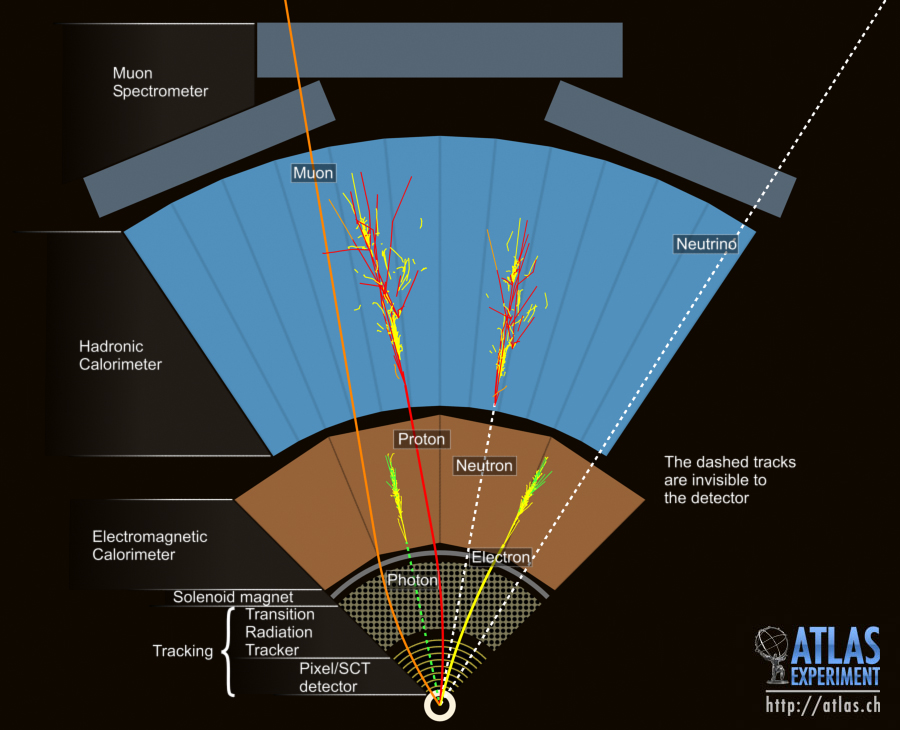
\includegraphics[width=.98\linewidth]{figures/LHC/ATLAS_Transverse.jpg}
    \caption{ Simplified representation of various particles traversing through different layers of ATLAS sub-detectors and leaving unique signatures \cite{ATLASTransverse}.\label{fig:ATLASTransverse}}
\end{figure}

\subsection{Trigger}
\label{subsec:TriggerATLAS}
The first step of particle and event reconstruction is selecting interesting high-energy events from a pool of lower-energy multiple-scattering signals. The high bunch crossing frequency of every $25$ ns results from a large amount of data making it physically impossible to store all events. ATLAS trigger system selects the events interesting for physics objects. 

ATLAS trigger consists of two levels, Level 1 (L1) trigger integrated into the hardware and high-level software trigger (HLT) \cite{TriggerSystemATLAS}. The L1 trigger is based on custom-built electronics, which uses signals from the calorimeters and muon trigger system (TGC and RPC) to identify event features such as electrons, photons, jets, taus, and missing energy. The L1 trigger reduces the $40$ MHz incoming collision data-rate corresponding to $25$ ns bunch crossing by a factor of $400$ to $100$ kHz output \cite{TriggerSystemATLAS}. The events accepted by the L1 trigger defines regions of interest (ROI), and HLT algorithms are run on these events to select ones with candidate physics objects and kinematic requirement. The software-based HLT trigger further reduces the data rate by almost a factor of 100 to $1.5$ kHz \cite{ATLAS}. With the combination of L1 and HLT trigger system, the data rate is reduced by $400,000$, and the selected events corresponding to data readout of $1.5$ GB are stored in the permanent storage. Figure \ref{fig:DAQ} shows the schematic of ATLAS's trigger and data acquisition system. 

\begin{figure}
    \centering
    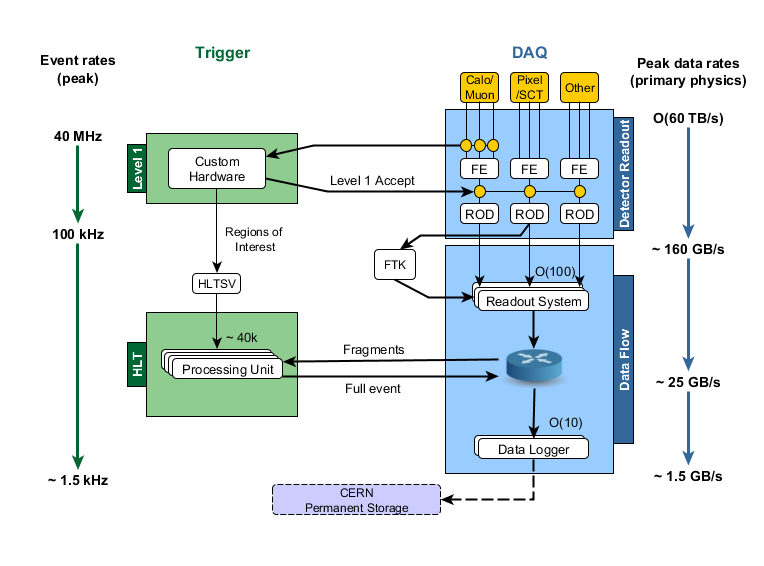
\includegraphics[width=.98\linewidth]{figures/LHC/DAQ_ATLAS.png}
    \caption{ Trigger and data acquisition system in ATLAS \cite{ATLAS_DAQ}.\label{fig:DAQ}}
\end{figure}

Physics object reconstruction discussed below converts the raw data output stored in permanent storage to physics objects used in physics analyses. 

\subsection{Tracks and Vertices Reconstruction}
\label{subsec:Tracking}
Tracking a charged particle is a critical step in reconstruction. The tracks of the charged particles play an essential role in momentum measurement, particle identification, and primary vertex reconstruction through the extrapolation of tracks to the interaction point. As the inner detector is closest to the beamline and comprises minimally ionizing detector material with high granularity, it plays a crucial role in track reconstruction. The ID magnetic field is homogenous, resulting in circular tracks of the charged particles. Five parameters define charged particle tracks; the ratio of charge and transverse momentum ($q/p_{T}$) defining the curvature; the distance of the closest approach to the primary vertex in $xy$-plane defining the transverse impact parameter ($d_{0}$), the longitudinal impact parameter ($z_{0}$) along the $z$-axis; the azimuthal angle ($\phi_{0}$) and the polar angle ($\theta_{0}$) of the particle direction at the closest approach point \cite{TrackingRun2_ATLAS}. Figure \ref{fig:TrackParameter} schematically shows the five-track parameters. 

\begin{figure}
    \centering
    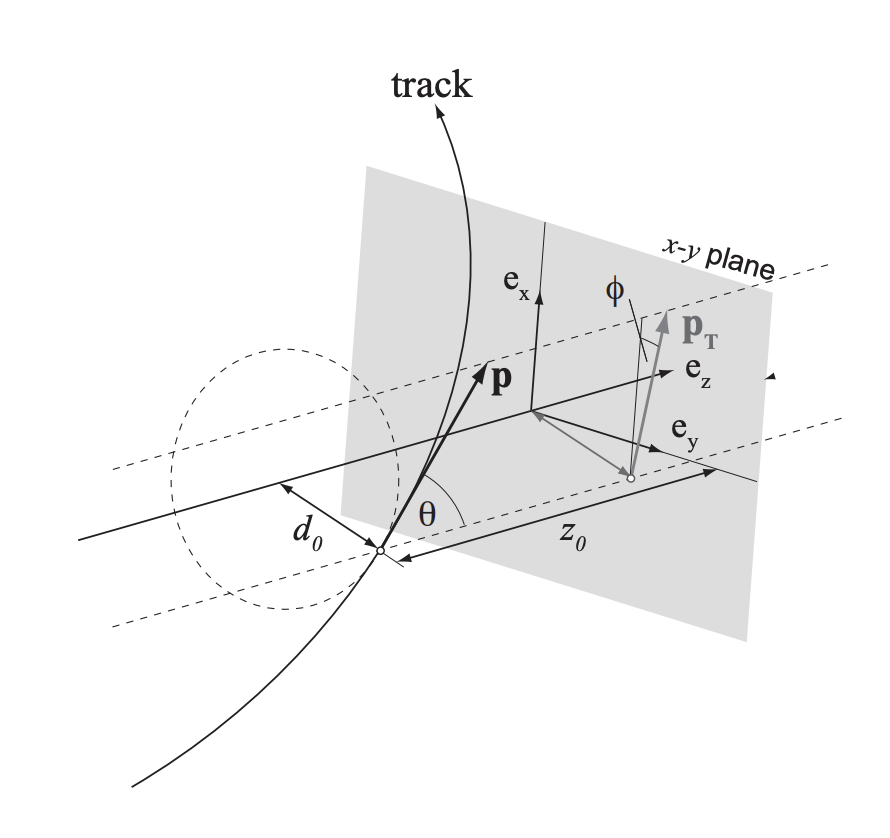
\includegraphics[width=.98\linewidth]{figures/LHC/TrackParameters.png}
    \caption{ Schematic showing the five-track parameters \cite{TrackParameterFig}.\label{fig:TrackParameter}}
\end{figure}

As shown by figure \ref{fig:TrackingOutline}, track reconstruction follows two different approaches used in Run-2; the primary \textit{inside-out} approach and the secondary \textit{outside-in} approach \cite{TrackingRun2_ATLAS}. The first step in the inside-out track reconstruction is the space point and drift circle formation, formed respectively by the clusters of signals from the silicon detectors and drift-circles hits in the TRT. Second, track seeds are formed from a collection of three silicon-detector space points and extrapolated to the outer layers by including the compatible clusters in the track trajectory. Once the track is formed, an ambiguity resolution algorithm is applied to reassign shared clusters to the track with a better match, and the final track candidate is fitted using a global $\chi^{2}$ method. The last step of inside-out track reconstruction is adding compatible TRT drift holes and refitting the tracks. 

\begin{figure}
    \centering
    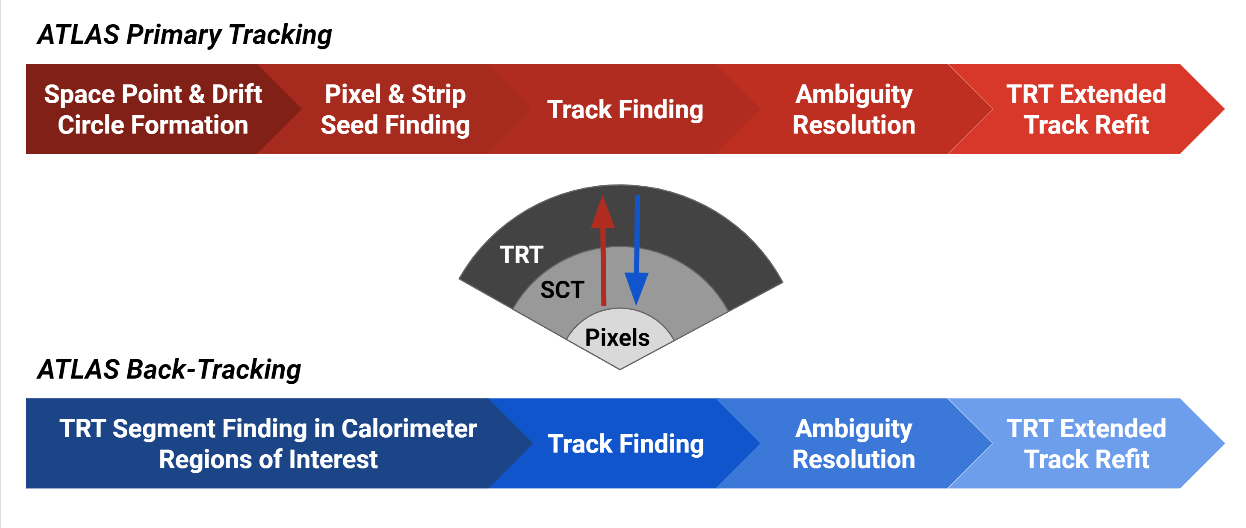
\includegraphics[width=.98\linewidth]{figures/LHC/trackingflowchart.png}
    \caption{schematic showing the two types of track reconstruction, primary inside-out and secondary outside-in. Taken from ATLAS Tracking CP group public tutorial \url{https://atlassoftwaredocs.web.cern.ch/trackingTutorial/idoverview/}. \label{fig:TrackingOutline}}
\end{figure}

The inside-out method is optimal for particles that minimally interact with the inner-detector material. However, secondary backtracking with an outside-in approach is needed for particles interacting with the inner detector, such as reconverted photons. In this approach, the track pattern recognition starts at the TRT in the regions of interest flagged by the electromagnetic calorimeter and backtracks to the silicon detectors. 

Tracks of the charged particle are extrapolated inward to the beamline and are assigned to vertices \cite{VertexReconstruction}. In most ATLAS analyses, including the one presented in this thesis, the space-point with the highest quadrature sum of track $p_T$ ($\sum_{track}{p_{T}^2}$) is identified as the primary vertex of an event.  

\subsection{Electrons}
\label{subsec:ParticleRecon_Elec}

\subsection{Muons}
\label{subsec:ParticleRecon_Muon}

\subsection{Jets}
\label{subsec:ParticleRecon_Jets}